\documentclass[12pt]{article}
\usepackage[a4paper,margin=2.5cm]{geometry}
\usepackage{tikz}
\usetikzlibrary{arrows.meta}

\begin{document}

\section*{Garis Bilangan Bilangan Bulat $-4$ sampai $4$}

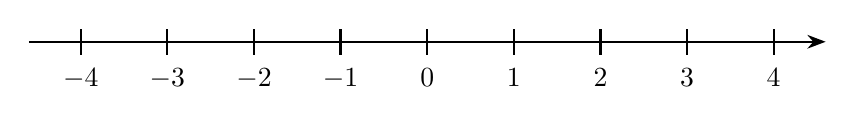
\begin{tikzpicture}[scale=1.1]
  \draw[thick,-{Stealth}] (-4.6,0) -- (4.6,0);
  \foreach \x in {-4,...,4} {
    \draw[thick] (\x,-0.15) -- (\x,0.15);
    \node[below] at (\x,-0.2) {$\x$};
  }
\end{tikzpicture}

\section*{Menunjukkan operasi $-3 + 5$ pada garis bilangan}

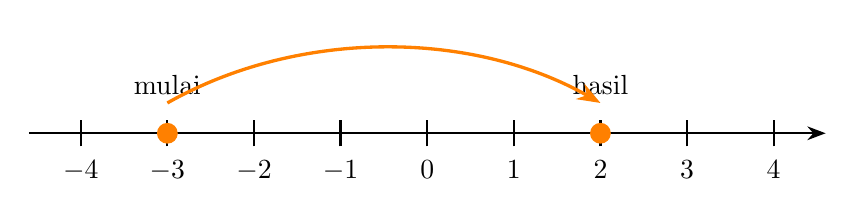
\begin{tikzpicture}[scale=1.1]
  \draw[thick,-{Stealth}] (-4.6,0) -- (4.6,0);
  \foreach \x in {-4,...,4} {
    \draw[thick] (\x,-0.15) -- (\x,0.15);
    \node[below] at (\x,-0.2) {$\x$};
  }
  % titik mulai dan hasil
  \fill[orange] (-3,0) circle (0.12);
  \fill[orange] (2,0) circle (0.12);
  \node[above=2mm] at (-3,0.15) {mulai};
  \node[above=2mm] at (2,0.15) {hasil};
  % panah lompatan
  \draw[very thick,orange,-{Stealth}] (-3,0.35)
    .. controls (-1.5,1.2) and (0.5,1.2) .. (2,0.35);
\end{tikzpicture}

\end{document}
